L'analyse syntaxique permet de vérifier que la structure d'un programme est bien en accord avec les règles de grammaire du langage. Par exemple, la grammaire de notre langage comporte une règle qui indique que le jeton \verb|<FD>| doit être suivi d'un jeton \verb|<NUMBER,>|. Le but de notre analyse ici est double~: vérifier que le programme est bien un programme de notre langage valide, mais également généré un arbre abstrait qui pourra facilement être analysé par notre analyseur sémantique.

Nous avons fait le choix d'utiliser GNU Bison (cf.~\ref{bison}) dans notre projet.

\subsection{Arbre abstrait}
Un arbre abstrait est une structure d'arbre dont chaque noeud feuille représente les opérandes des opérations contenues sur les autres noeuds. Cet arbre peut être considéré comme une forme de code intermédiaire, et peut être interprété très facilement en interprétant pour chaque noeud, les sous-arbres et en appliquant l'opération du noeud courant.

\begin{lstlisting}[language=Stibbons,label=arbre-code,caption=Exemple de code Stibbons]
  agent turtle (a) {
    teleport(50,50,0)
    fd a
  }

  b = 18
  repeat b {
    if(b == 18) {
      new turtle(b)
    }
    else {
      new turtle(3)
    }
    b = b - 1
  }
\end{lstlisting}

\begin{figure}[h]
\centering
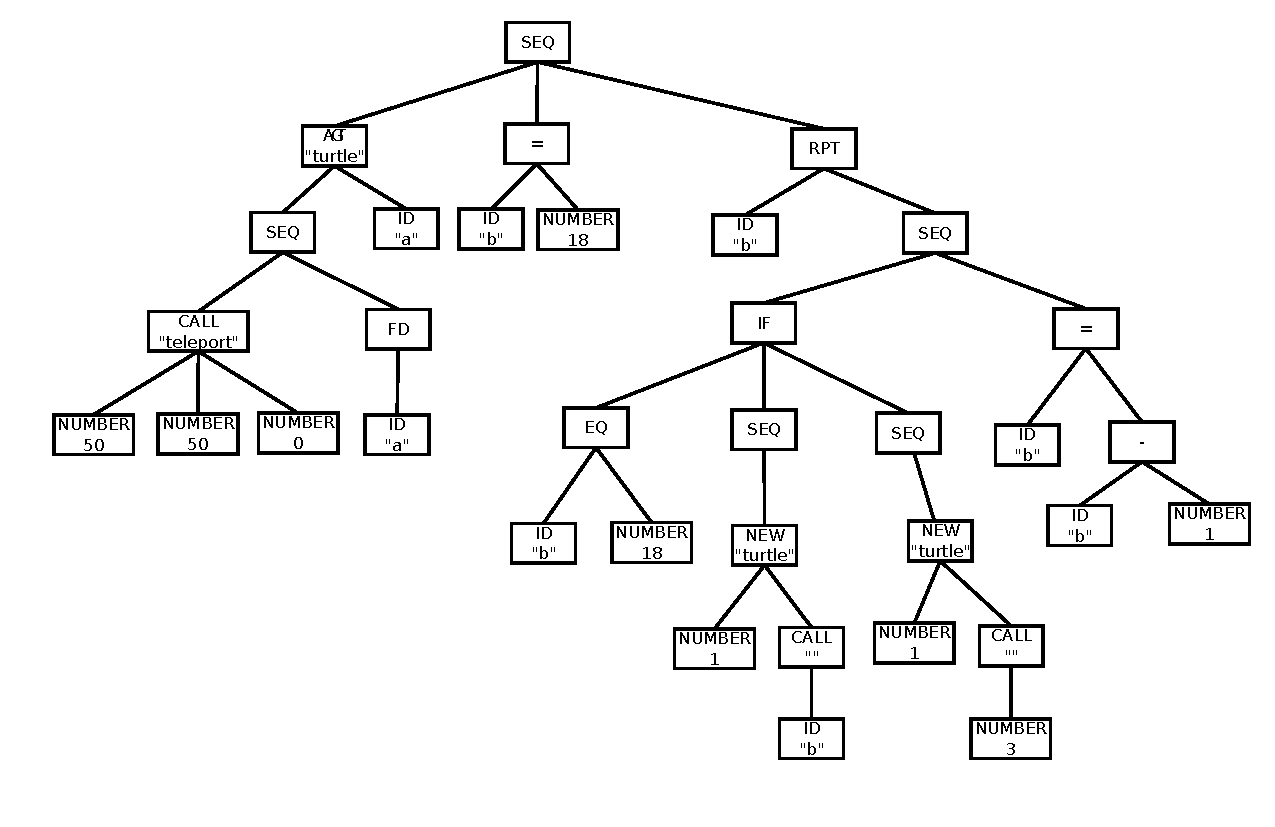
\includegraphics[scale=0.8]{doc/report/img/arbre-abstrait}
\caption{\label{arbre-abstrait} Arbre abstrait généré lors de l'analyse du code \ref{arbre-code}}
\end{figure}

L'avantage de générer un tel arbre est qu'il est bien plus rapide d'effectuer un parcours d'arbre à chaque interprétation plutôt que de refaire une analyse syntaxique à chaque fois.

\subsection{Fonctionnement}

\subsubsection{Analyse syntaxique LALR}
